\section*{Problem 2: Inverse Kinematics} \label{Sec: Problem 2: Inverse Kinematics}


Now, given the joint angles $\theta_1$ and $\theta_2$ we can determine the end-effector coordinates $x$ and $y$.\\
In order to command the robot to move to location $B$ we need the inverse; that is, we need
the joint variables $\theta_1$ and $\theta_2$ in terms of the $x$ and $y$ coordinates of $B$.
This is the problem of \textbf{Inverse Kinematics}. In other words, if we know $x$ and $y$ in the forward kinematic equations
(\ref{eq:positionX}-\ref{eq:orientation}), we wish to use this to make an equation for each joint angle, such that if we input $x$ and $y$
in our equations, the correct joint values will be found.\\
A solution may not be easy to find nor is there a unique solution of the \textbf{Inverse Kinematics} in general.
We can see, for example, in the case of a two-link planar mechanism that there may be no
solution, if the given $(x,y)$ coordinates are out of reach of the manipulator.
If the given $(x,y)$ coordinates are within the manipulator’s reach there may be two solutions as shown
in Figure \ref{fig:Figure1_26}, the so-called \textbf{elbow up} and \textbf{elbow down} configurations, or there may be
exactly one solution if the manipulator must be fully extended to reach the point. There
may even be an infinite number of solutions in some cases.

\begin{figure}[H]
	\centering
	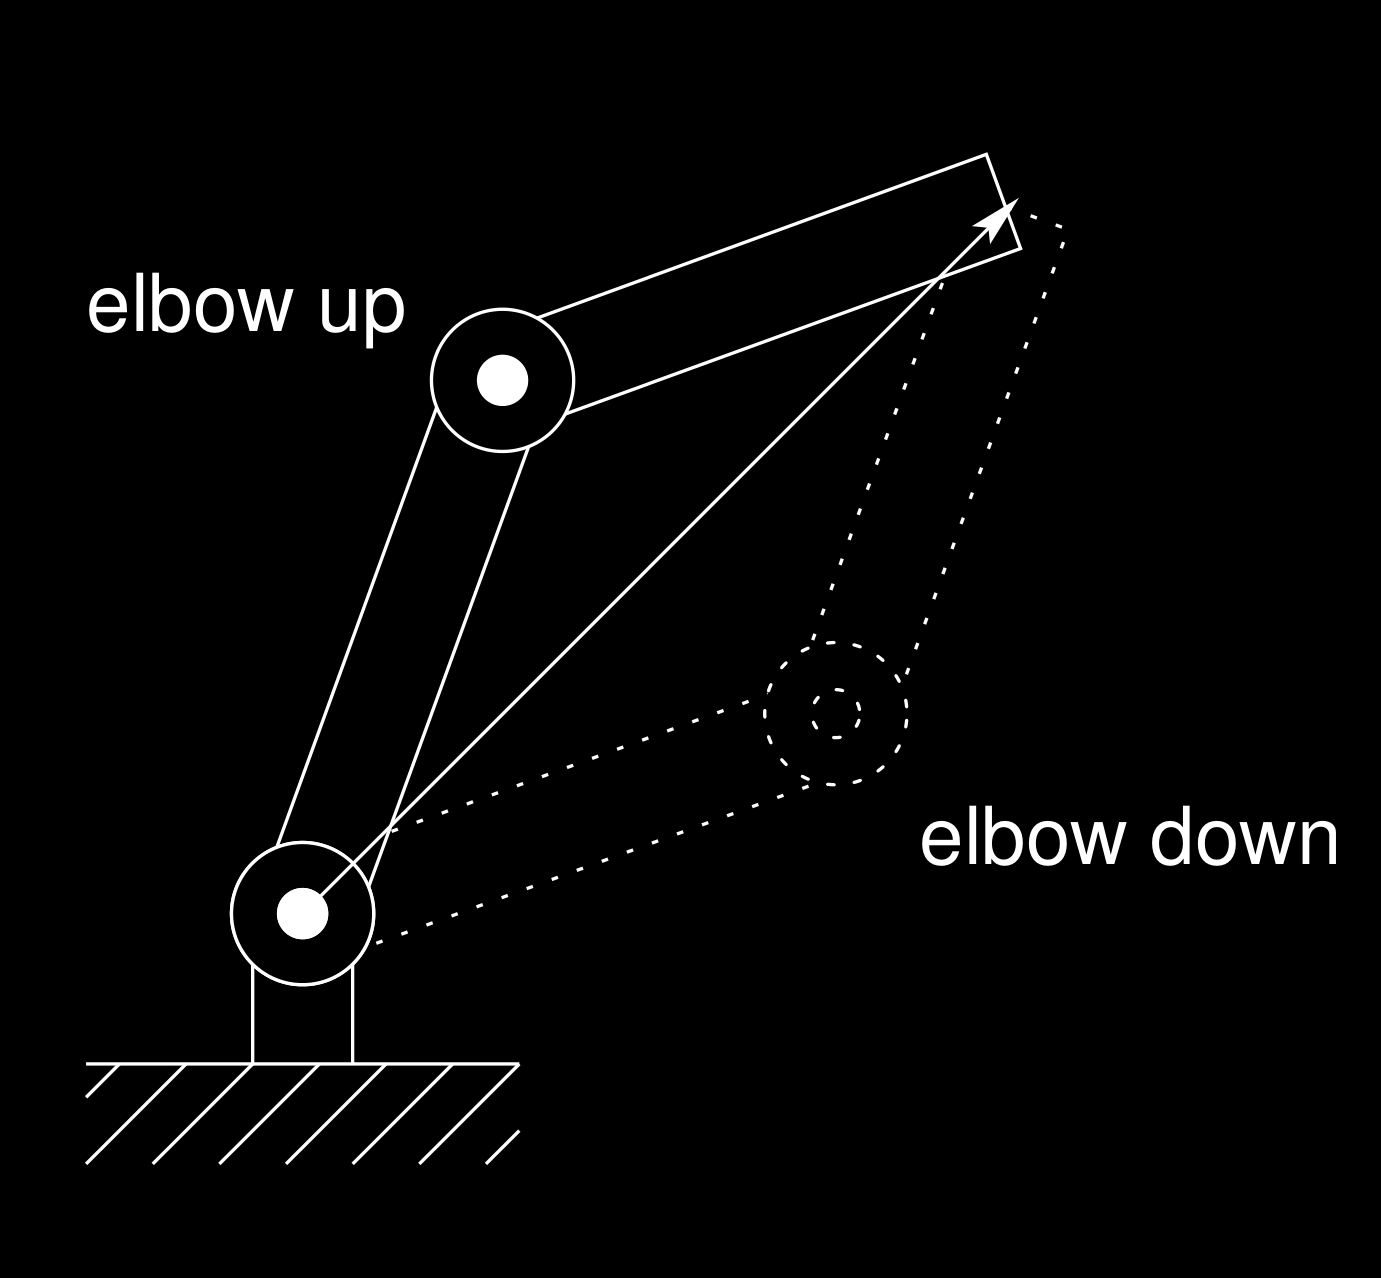
\includegraphics[width=1\textwidth]{img/Figure1_26.png}
	\caption{Multiple inverse kinematic solutions.}
	\label{fig:Figure1_26}
\end{figure}

Consider now the diagram of Figure \ref{fig:Figure1_27}.

\begin{figure}[H]
	\centering
	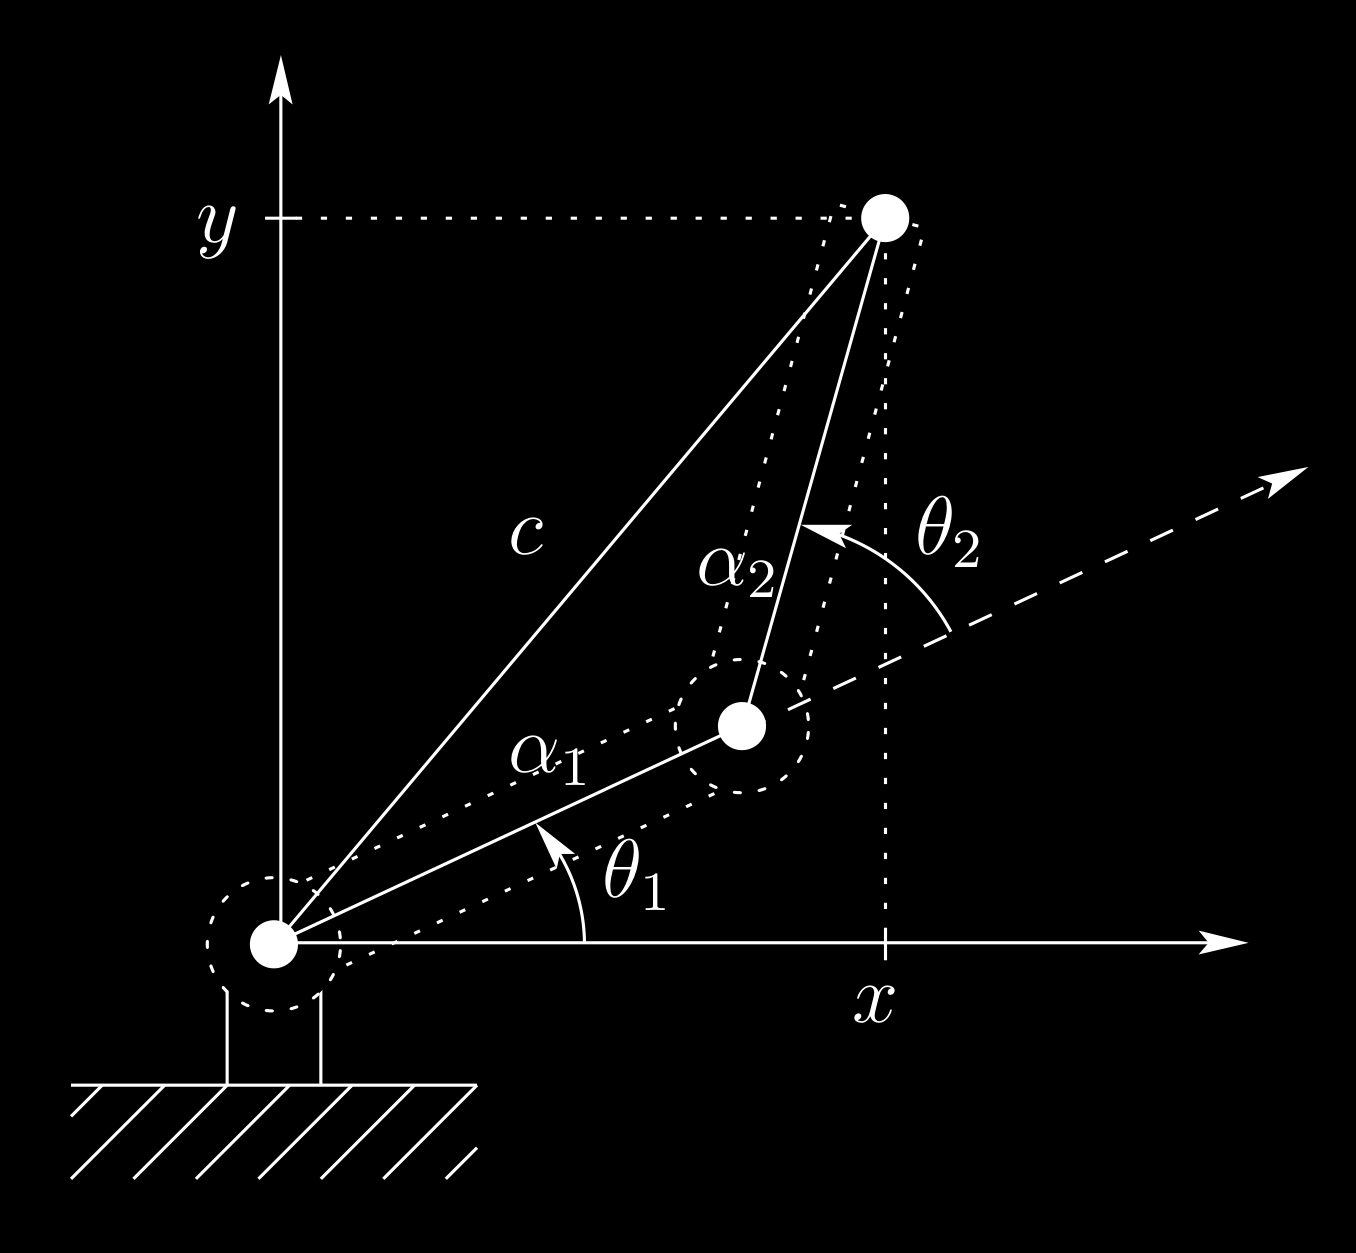
\includegraphics[width=0.7\textwidth]{img/Figure1_27.png}
	\caption{Solving for the joint angles of a two-link planar arm.}
	\label{fig:Figure1_27}
\end{figure}

By using the \textbf{Law of Cosines} we can derive (simply by putting the different lengths above into the definition) an equation containing $\theta_2$:

\begin{equation} \label{eq:LawOfCos}
	cos(\theta_2) = \frac{x^2 + y^2 - \alpha_1^2 - \alpha_2^2}{2\alpha_1\alpha_2} = D
\end{equation}

Furthermore, notice that if we use some of our well-known \emph{Pythagorean Identities}, $\theta_2$ can be found by:

\begin{equation} \label{eq:Theta2}
	\theta_2 = \tan^{-1}{\bigg(\frac{\pm\sqrt{1-D^2}}{D}\bigg)}
\end{equation}

There are several ways of solving the \textbf{Inverse Kinematics} equations, but the advantage of this approach is that both the \textbf{elbow-up} and \textbf{elbow-down} solutions are recovered by choosing the positive and negative signs in (\ref{eq:Theta2}), respectively.

Moreover, it can be shown that $\theta_1$ is given as

\begin{equation} \label{eq:Theta1}
	\theta_1 = \tan^{-1}{\bigg(\frac{y}{x}}\bigg) - \tan^{-1}{\bigg(\frac{\alpha_2\sin{\theta_2}}{\alpha_1 + \alpha_2\cos{\theta_2}}\bigg)}
\end{equation}

Notice that the angle $\theta_1$, depends on $\theta_2$. This makes sense physically since we would
expect to require a different value for $\theta_1$, depending on which solution is chosen for $\theta_2$.
The derivation and specific details related to the equations stated above are covered thoroughly later on in the book.
